Die Ortsänderung in jedem Abschnitt ist die Fläche unter dem $v(t)$-Graphen, unter der Achse negativ. Der Graph schneidet die $t$-Achse in der Mitte zwischen \tOneO\ und \tTwoO.
\begin{abcliste}
\abc Solange $v>0$ ist, bewegt sich der Körper vorwärts; danach rückwärts. Am weitesten vorne ist er beim Vorzeichenwechsel von $v$, bei
\begin{align}
 t_\mathrm{U} &= \tTurnF = \tTurn \approx \result{\tTurnP{0}{1}}
\end{align}
Bis dahin ist die Fläche ein Rechteck bis \tOneO\ und ein Dreieck:
\begin{align}
 s_1 &= \sOneF = \vNull\cdot\tOne = \sOne \\
 s_\mathrm{max} &= \sMaxF = \sMax \approx \result{\sMaxP{0}{1}}
\end{align}
\abc Von \tTurnP{0}{1}\ bis \tTwoO\ kommt das Dreieck unter der Achse dazu ($-\SI{1}{\meter}$), bei \tTwoO\ ist der Körper also wieder bei $s_2 = \sTwoP{0}{1}$. Danach:
\begin{align}
 s(t_\mathrm{e}) &= \sEndF = \sEnd \approx \result{\sEndP{0}{1}}
\end{align}
Wo $v$ konstant ist, ist $s(t)$ eine Gerade (Steigung $+2$ bzw. $-2$); wo $v$ linear abnimmt, ist $s(t)$ eine nach unten gekrümmte Parabel mit dem Maximum (waagrechte Tangente) bei \tTurnP{0}{1}. Der Graph hat keine Knicke, weil $v$ keine Sprünge hat.
\begin{center}
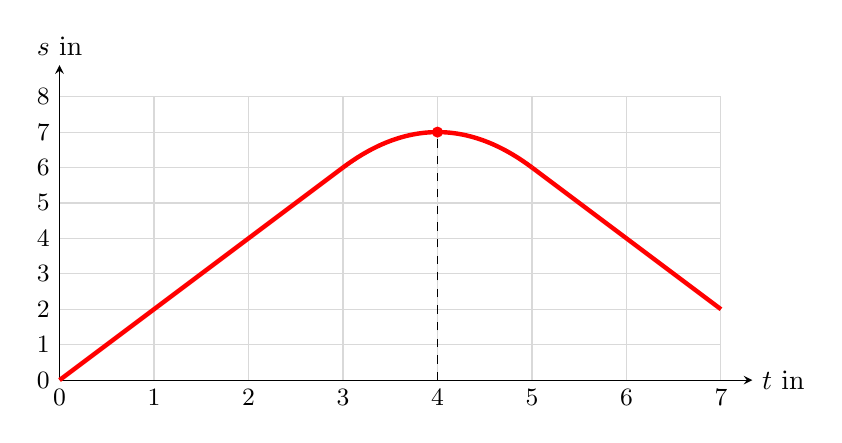
\begin{tikzpicture}[>=stealth, x=1.2cm, y=0.45cm]
 \draw[gray!30] (0,0) grid[xstep=1, ystep=1] (7,8);
 \draw[->] (0,0) -- (7.333,0) node[right] {$t$ in \si{\second}};
 \draw[->] (0,0) -- (0,8.889) node[above] {$s$ in \si{\meter}};
 \foreach \tk in {0,1,2,3,4,5,6,7} \node[below] at (\tk,0) {\small $\tk$};
 \foreach \yk in {0,1,2,3,4,5,6,7,8} \node[left] at (0,\yk) {\small $\yk$};

 \draw[ultra thick, red] (0,0) -- (3,6);
 \draw[ultra thick, red, domain=3:5, samples=40] plot (\x, {6+2*(\x-3)-(\x-3)*(\x-3)});
 \draw[ultra thick, red] (5,6) -- (7,2);
 \draw[dashed] (4,0) -- (4,7);
 \fill[red] (4,7) circle (2pt);
\end{tikzpicture}
\end{center}
\end{abcliste}
